\chapter[Pulse feature extraction]{\uppercase{Pulse feature extraction}}
\label{chap:four}

Different from the traditional pulse diagnosis, the digitized wrist
pulse in the paper is an objectified, precisely quantified,
standardized and automated pulse signal. As an important issue in
pattern classification field, feature extraction directly affects the
design and performance of classifier. If the features extracted from
distinct classes sharply differ from one another, it is easy to design a
high discrimination classifier. Thus, Thus, how to extract features from the
sample effectively is a tremendous step in pulse patter
classification process. \todo{时域频域}

\section{Time-domain features}
\subsection{Time-domain features and its physiological significance}
A complete cycle of pulse waveform consists of an ascending limb and a
descending limb, shown as Figure~\ref{fig:waveform}. The ascending limb results from the systole activity:  
When systole occurs, the left ventricle ejects blood to the aorta in the sphygmic
period; The increase of blood pressure causes the elastic expansion
of aorta, that leads to the displacement of vascular wall. Likewise,
the descending limb occurs in the late systole period when the blood
ejection rate slows down; The pressure in the aorta decreases and then the
vascular wall shrinks. 
The minimum point as point 3
in the figure is called dicrotic notch. In physiological view, it
denotes a small downward deflection in the arterial pulse or pressure
contour immediately following the closure of the semilunar valves and
preceding the dicrotic wave, sometimes used as a marker for the end of
systole or the ejection period. The secondary peak in the figure is
called tidal wave while the third peak is called dicrotic wave. 
These peaks and troughs construct an entire pulse cycle. 
\begin{figure}[htbp]
    \begin{center}
        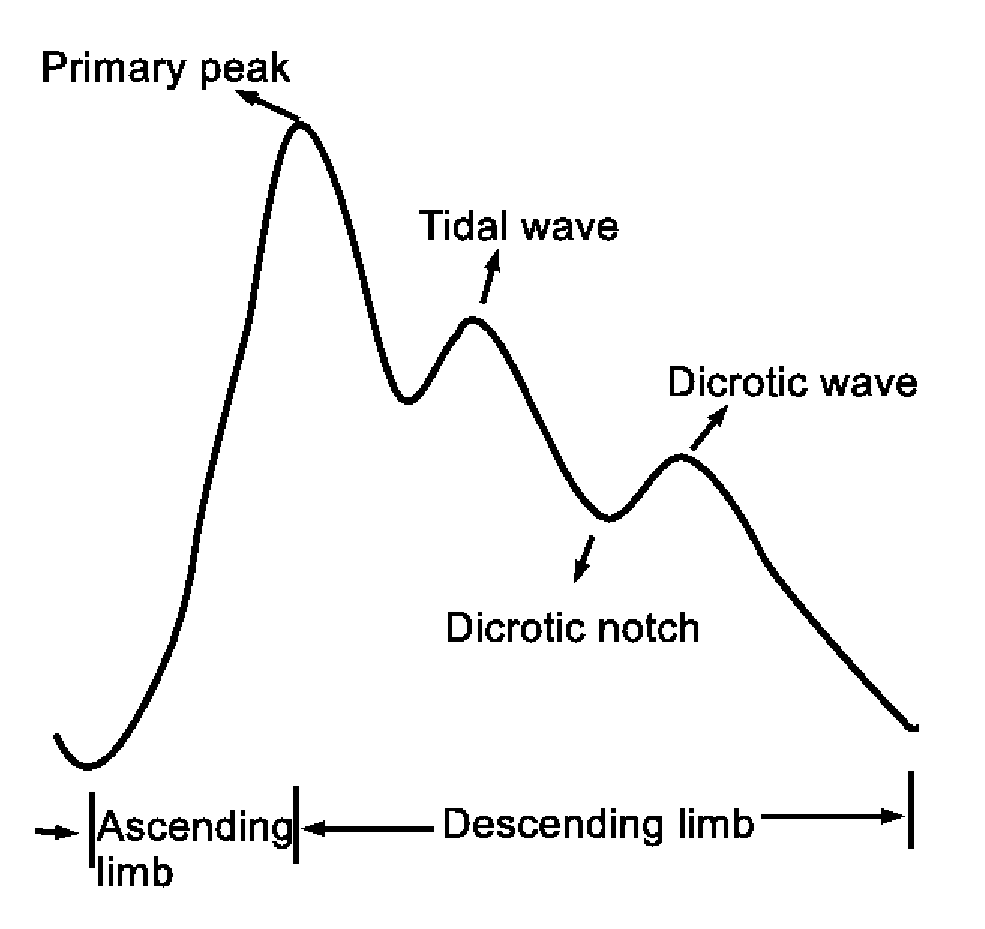
\includegraphics[width=0.4\textwidth]{pulsewaveform}
    \end{center}
    \caption{The basic structure of pulse waveform}
    \label{fig:waveform}
\end{figure}

The pulse image is the locus of vascular pulsation, so it has a
certain amount of significance. It integrates the information of 
vibration in cardiac ejection period and the pulse propagation along
vessels, which is reflected as the curve and inflection point in pulse
image. Some critical parameter illustrated in Figure~\ref{fig:timefeatures} and its
explanation could reveal the physiological meaning of pulse image.
\begin{figure}
    \centering
    \subfloat[shape
    features]{\label{fig:shape}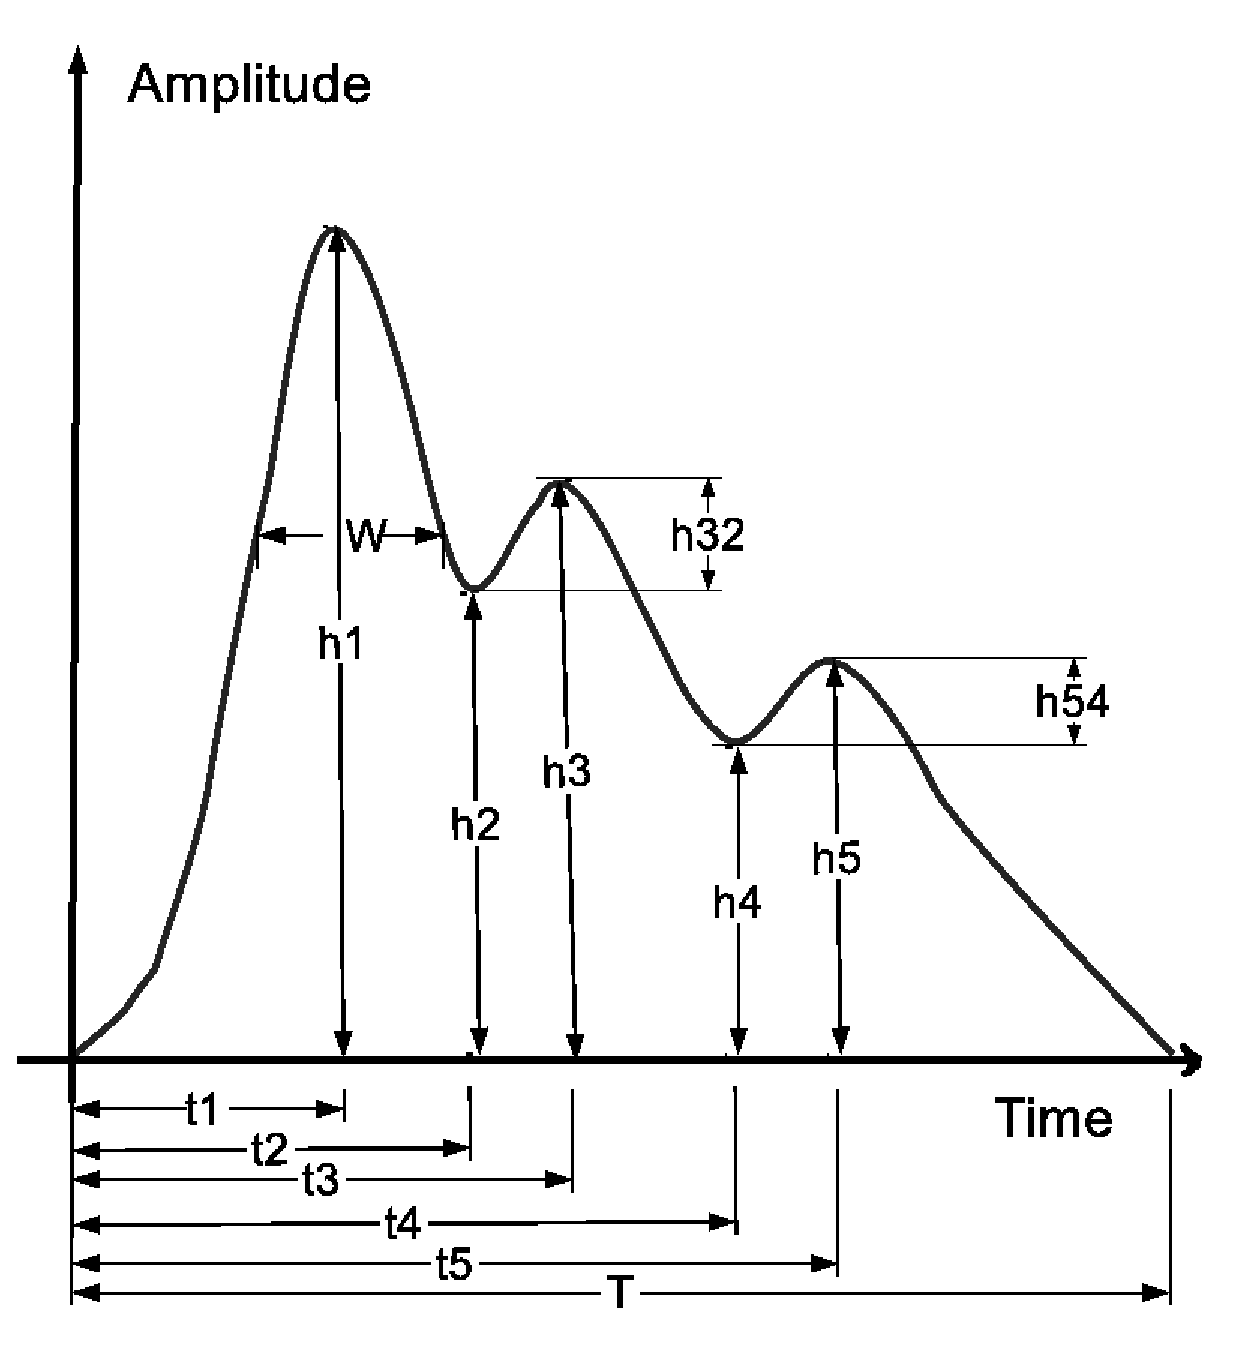
\includegraphics[width=0.3\textwidth]{shapefeatures}}
    \subfloat[area
    features]{\label{fig:area}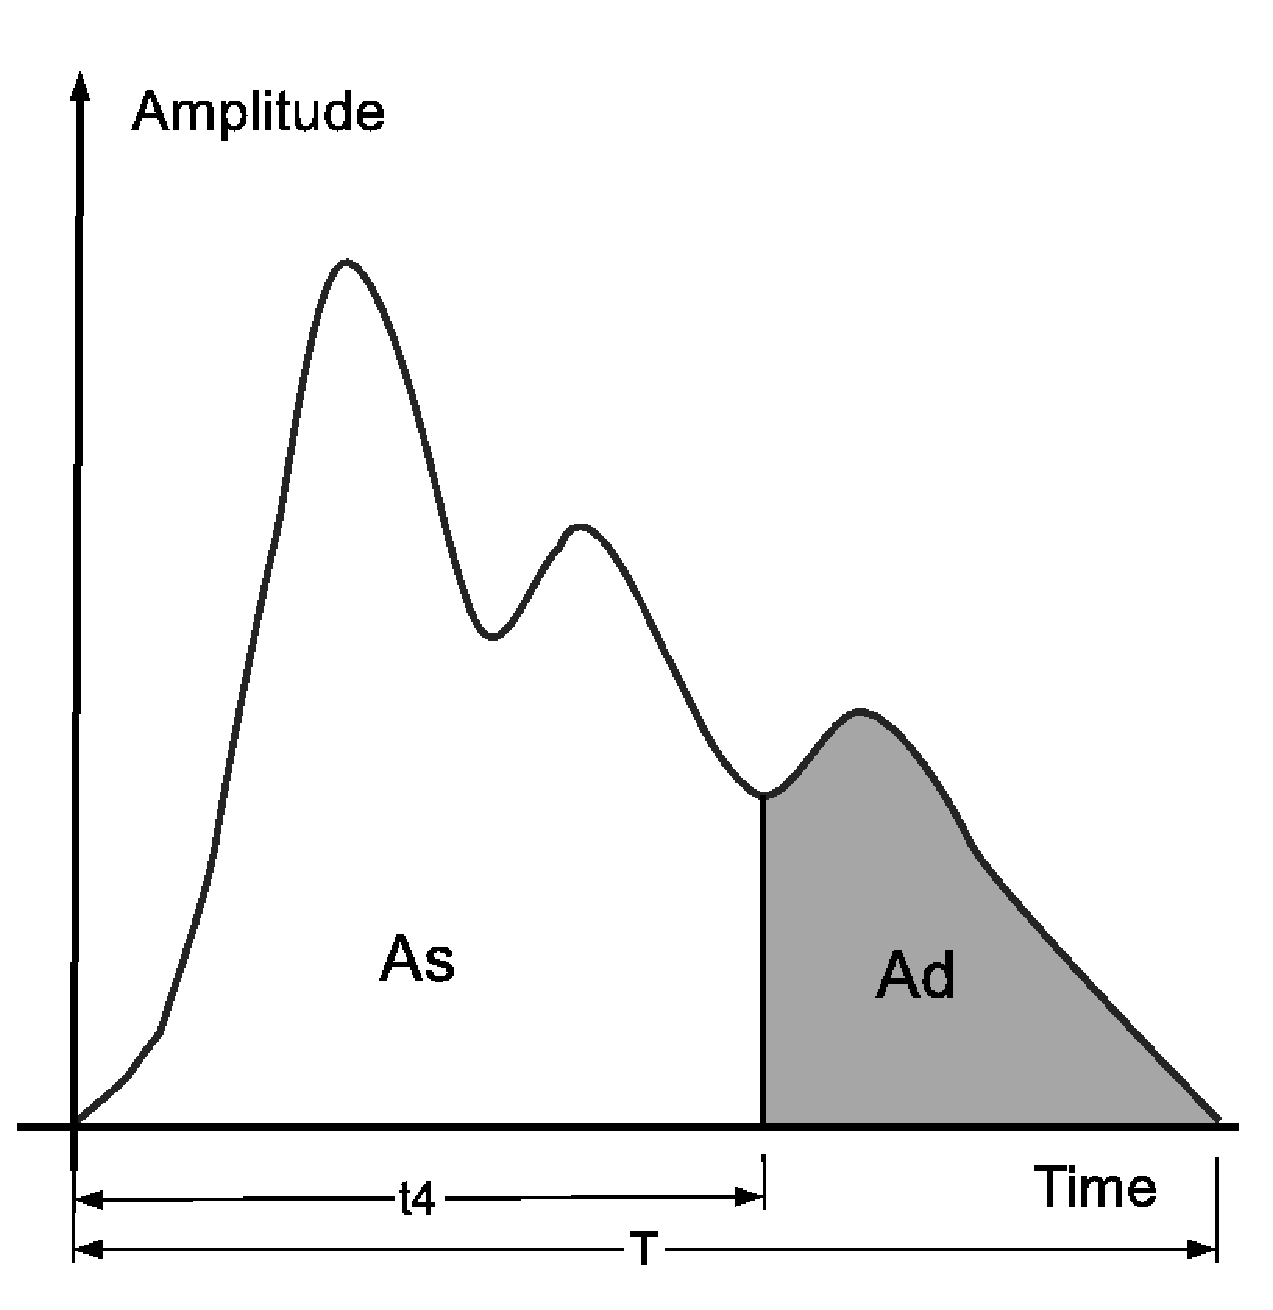
\includegraphics[width=0.3\textwidth]{areafeatures}}
    \caption{Time-domain features}
    \label{fig:timefeatures}
\end{figure}

These time-domain features represent special meanings as follows:
\begin{description}
    \item[h1:] The amplitude of primary wave. It is the height from
        the primary peak to x-axis (time base). The height reflects
        the sphygmic capacity of left ventricle and the arterial
        adaptability. Generally speaking, the stronger of the two
        capacity, the higher h1 is. Otherwise, the smaller h1 is. 
    \item[h2:] The amplitude of primary notch. It is the trough
        height between the primary wave and tidal wave.
    \item[h3:] The amplitude of tidal wave, i.e. the distance from the
        peak of tidal wave to x-axis. It reflects the arterial
        elasticity and peripheral resistance state. The amplitude h3
        would increase either if the arterial wall tension arises or
        if vascular sclerosis occurs or if the surrounding resistance
        arises. The elevation of tidal wave is often accompanied with
        the advance of time phase, which demonstrates a faster
        propagation rate of reflected wave in a state of high arterial
        tension and high resistance. 
    \item[h32:] The peak height of tidal wave. 
    \item[h4:] The amplitude of dicrotic notch, i.e. the distance
        between the trough of dicrotic notch to the x-axis, 
        corresponding to the diastolic pressure. It relates with arterial
        peripheral resistance and the aorta valve function. In
        general, h4 increases along with the rise of peripheral
        resistance. Otherwise, h4 decreases. 
    \item[h5:] The amplitude of dicrotic wave, i.e. the distance
        from the peak of dicrotic wave to the line across the trough
        of dicrotic notch, parallel to x-axis. The amplitude mainly
        reflects the aortic elasticity and aortic valve function. When
        the aortic adaptability diminishes or the aortic valve
        scleroses, h5 will eliminate correspondingly.  
    \item[h54] The peak height of dicrotic wave.
    \item[T] The time of a cycle, a.k.a. pulsation period,
        corresponding to a cardiac cycle of left ventricle. However,
        the pulse and ECG cardiac cycle will not be the same at the
        time of auricular fibrillation or extrasystole. 
    \item[t1] The time from start point of a cycle to the peak point,
        corresponding to rapid left ventricle ejection period. 
    \item[t2] The time from start point to the primary notch.
    \item[t3] The time from start point to the tidal wave peak point
    \item[t4] The time from start point of a cycle to dicrotic
        notch point, corresponding to the systole period of left
        ventricle. 
    \item[t5] The time from start point to the dicrotic wave peak
        point. 
    \item[W] The dominant peak width, where the junction height is
        defined as 2/3 of h1.
    \item[As] Area in systole period, related to the ejected blood volume. 
    \item[Ad] Area in diastole period.
    \item[PeakNum] the number of peaks. 
\end{description}

As can be seen from Figure~\ref{fig:keypoint}, the detection of key points A,
B, C, D, E, F is the critical step in time-domain features. Only if
these points are detected, can the calculation of the time-domain
relative features be launched. 
\begin{figure}[htpb]
    \begin{center}
        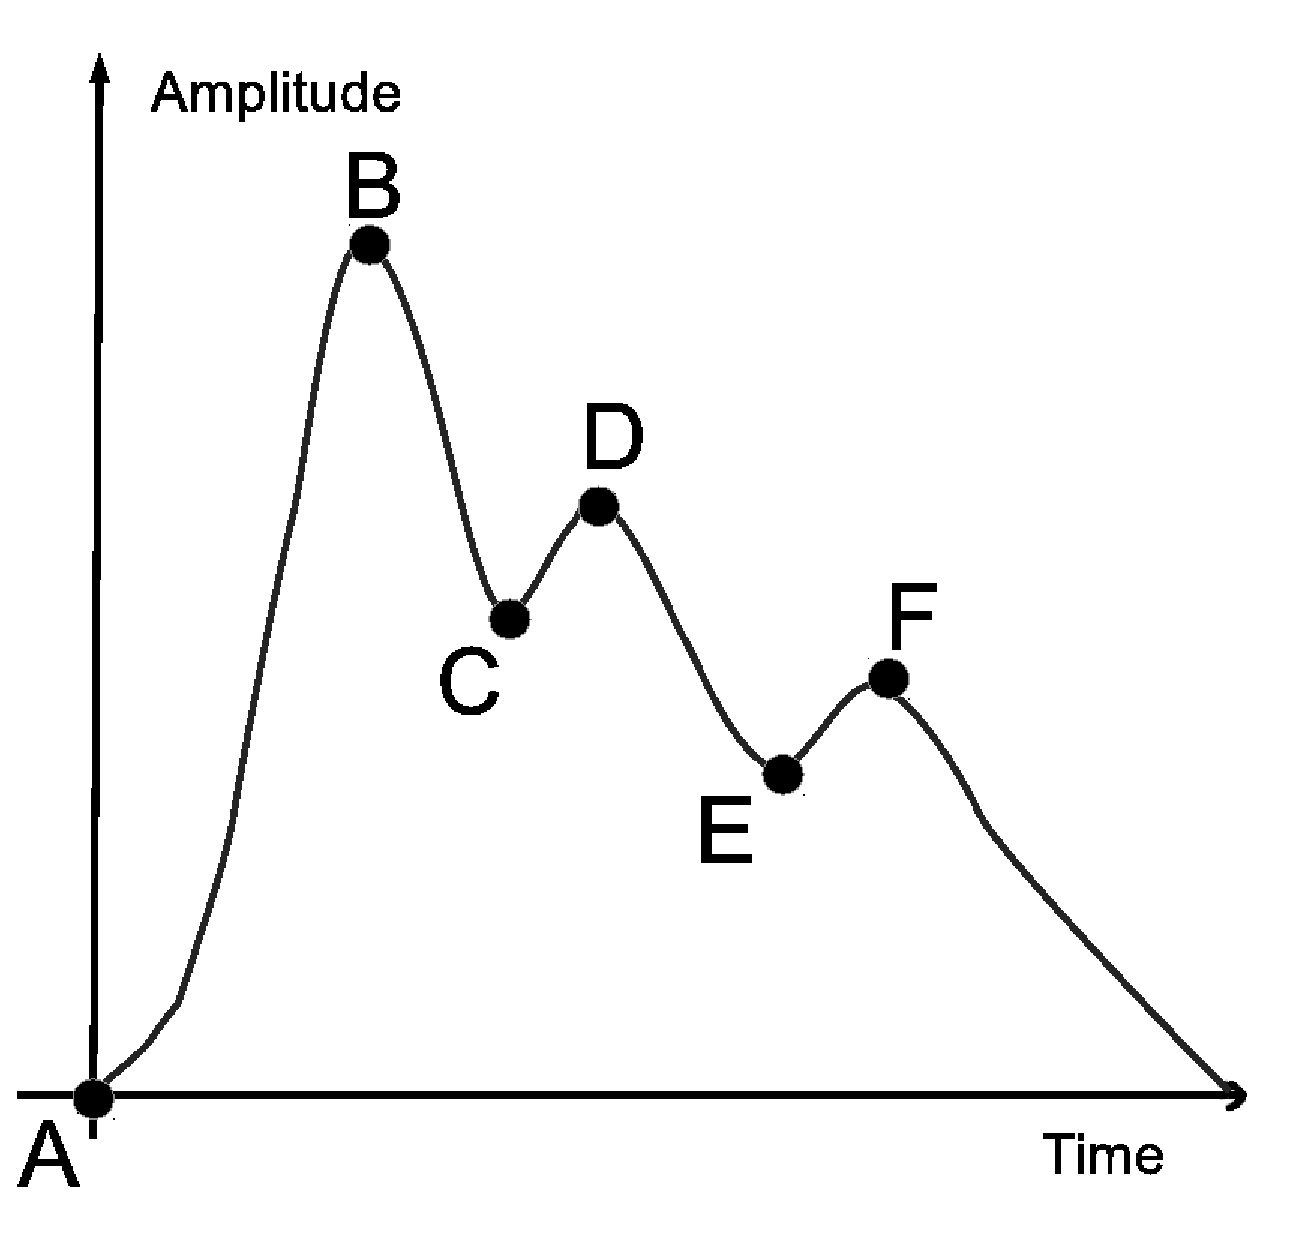
\includegraphics[width=0.4\textwidth]{keypoint}
    \end{center}
    \caption{The key points in a pulse cycle}
    \label{fig:keypoint}
\end{figure}
In fact, it can be seen that the
feature extraction is equivalent to the search of peak/trough points,
where the first derivative is zero. A derivative-based zero-cross
analysis is utilized for this purpose, and the peak search method are as follows:
\begin{enumerate}[(1)]
    \item Let the peak search range to be $0.85T$, which saves computing
        time. It is mainly because
        all peaks are located within the first 85\% of the waveform
        range after careful inspection. It is illustrated as the blue
        dotted line in Figure~\ref{fig:keypointsdetect}.
    \item Calculate the derivative of the signal, $d(t)$, as displayed
        in Figure~\ref{fig:firstderivative}. Since the pulse
        waveform is actually a sampled discrete signal, difference
        operation is applied in this case. There are many finite difference
        methods, e.g. forward difference $\Delta f(x)=f(x+1)-f(x)$,
        backward difference $\nabla f(x)=f(x)-f(x+1)$, central
        difference $\delta[f](x)=f(x+\frac{1}{2}h)-f(x-\frac{1}{2})$.
        The paper choose a eclectic approach between backward
        difference and forward difference. The form is given as:
        \begin{equation}
            x'_i=\left\{ 
            \begin{array}{ll}
                \frac{(x_i-x_{i-1})+(x_{i+1}-x_{i-1})/2}{2}, & i=2,\ldots,N-1\\
                x'_2, & i=1\\
                x'_N, & i=N-1\\
            \end{array} \right.
            \label{equ:1stdiff}
        \end{equation}
        \begin{equation}
            x''_i=\left\{ 
            \begin{array}{ll}
                \frac{(x'_i-x'_{i-1})+(x'_{i+1}-x'_{i-1})/2}{2}, &
                i=2,\ldots,N-1\\
                x''_2, & i=1\\
                x''_N, & i=N-1\\
            \end{array} \right.
            \label{equ:2nddiff}
        \end{equation}
        This eclectic derivative estimation method has advantages over
        the traditional method, which considers only two points, in
        robustness and generality. The method considers three points
        at meantime and is more accurate. Because this difference
        method makes no sense on the first point and the last point,
        let the derivative of second point and the one of penultimate
        point approximate to them, respectively.  
    \item Search the zero-cross points $d_i\;(i=1\,to\,5)$ in
        the derivative figure, and determine the revelent $h_i$ and
        $t_i$. 
    \item Search the first two points $P_1$ and $P_2$ whose amplitude equals to
        $2/3h_i$ within $[0,t_1]$ and $[t_1, t_2]$, respectively, and
        calculation the width $W=t(P_1)-t(P_2)$.
\end{enumerate}
\begin{figure}
    \centering
    \subfloat[The detected key
    points]{\label{fig:keypointsdetect}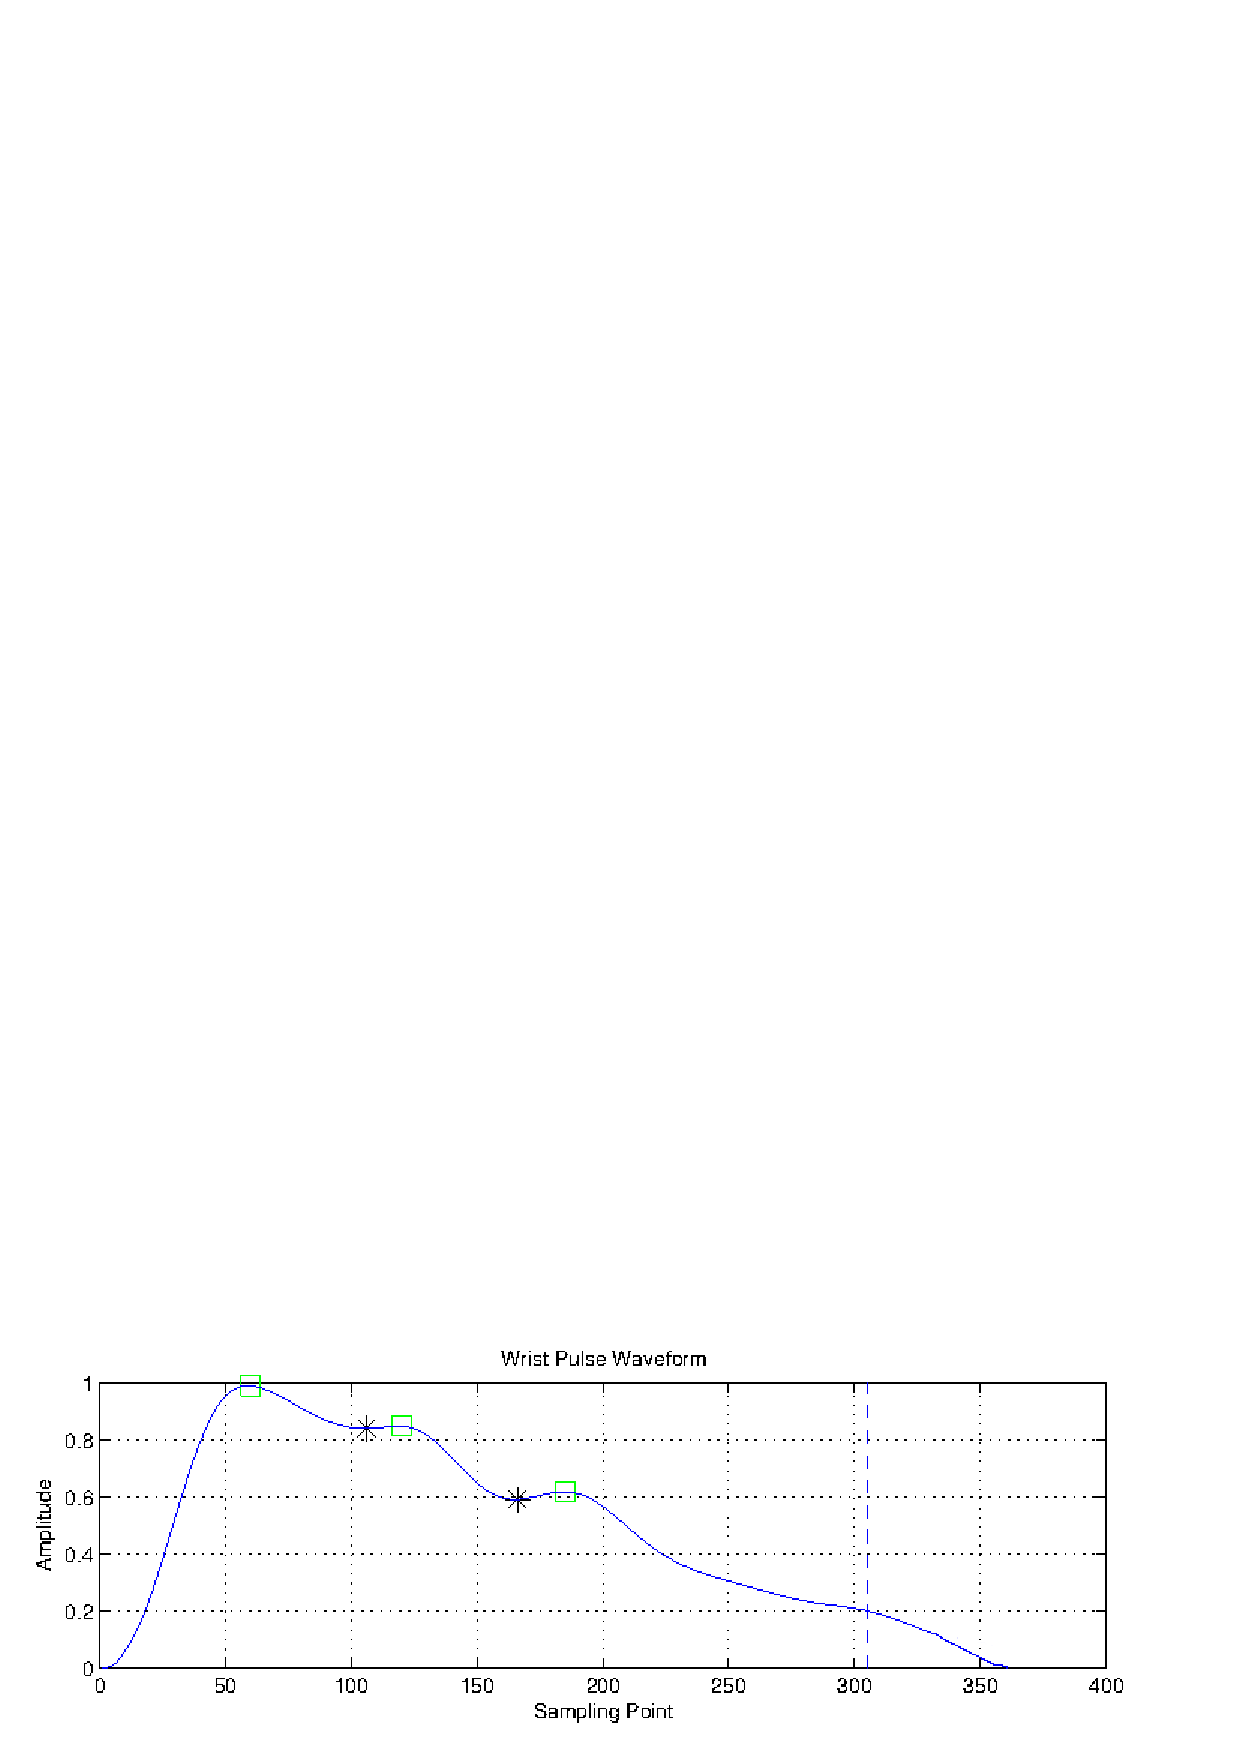
\includegraphics[width=0.6\textwidth]{keypointsdetected}}\\
    \subfloat[The first derivative of pulse
    waveform]{\label{fig:firstderivative}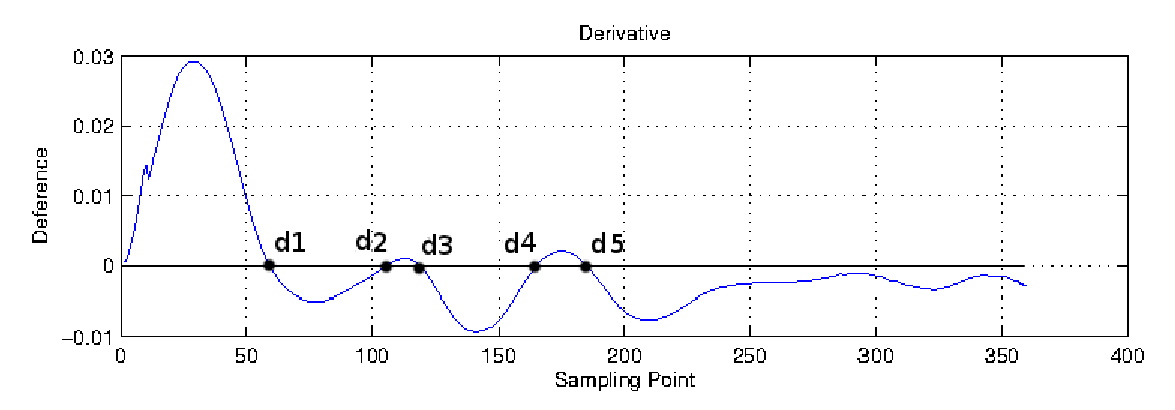
\includegraphics[width=0.6\textwidth]{firstderi}}
    \caption{The key points detected by the algorithm}
    \label{fig:keypointsgroup}
\end{figure}


Of course, these shape features may differ person by person. In
practice, for some pulse waveforms, the tidal wave may ``disappear'',
i.e. the tidal wave is so close to the primary peak that the height of
primary notch is still greater than the peak tidal wave. The
\emph{Xian Mai} is a typical case, shown in Figure~\ref{fig:xianmai}.
For such case, the zero-crossing points for $h_2$ and $h_3$ is missed.
To solve the issue, the paper introduces a \emph{tolerance} $\delta$ to find
the hidden pseudo trough and peak. An automated moving line
crossing point search is performed to get pseudo $h_2$ and $h_3$, which
equivalent to the search of points $d_1$ and $d_2$. The algorithm is
as follows:
\begin{enumerate}[(1)]
    \item Let the search range from $d_1$ to $d_4$;
    \item Find the maximum point within the range in the first-order
        deference, i.e. find all the
        zero-cross from positive to negative in the second-order
        deference (Figure~\ref{fig:2nddiff}). The point $d_{2(3)}$ in
        the first-order difference corresponds to its derivative point
        $dd_23$ in the second-order difference. 
    \item Check the validity of $d_{2(3)}$. 
        \begin{enumerate}[a)]
            \item If the maximum is upper than the dotted line
                $-\delta$ in the first-order difference
                (Figure~\ref{fig:1stdiff}, i.e. $d_{2(3)}<0 \; \& \;
                d_{2(3)} > -\delta$, then the sampling point $d_{2(3)}$ is a valid
                hidden peak of tidal wave.
            \item If the maximum is lower than the dotted line
                $-\delta$ in the first-order difference, i.e.
                $d_{2(3)}<-delta$, then the sampling point
                $d_{2(3)}$ is ignored.
        \end{enumerate}
\end{enumerate}

\begin{figure}[htbp]
    \begin{center}
        
\includegraphics[width=0.5\textwidth]{xianmai}
    \end{center}
    \caption{Xian Mai: hidden tidal wave}
    \label{fig:xianmai}
\end{figure}

\begin{figure}
    \centering
    \subfloat[The pulse waveform of hidden tidal
    wave]{\label{fig:hiddenpulse}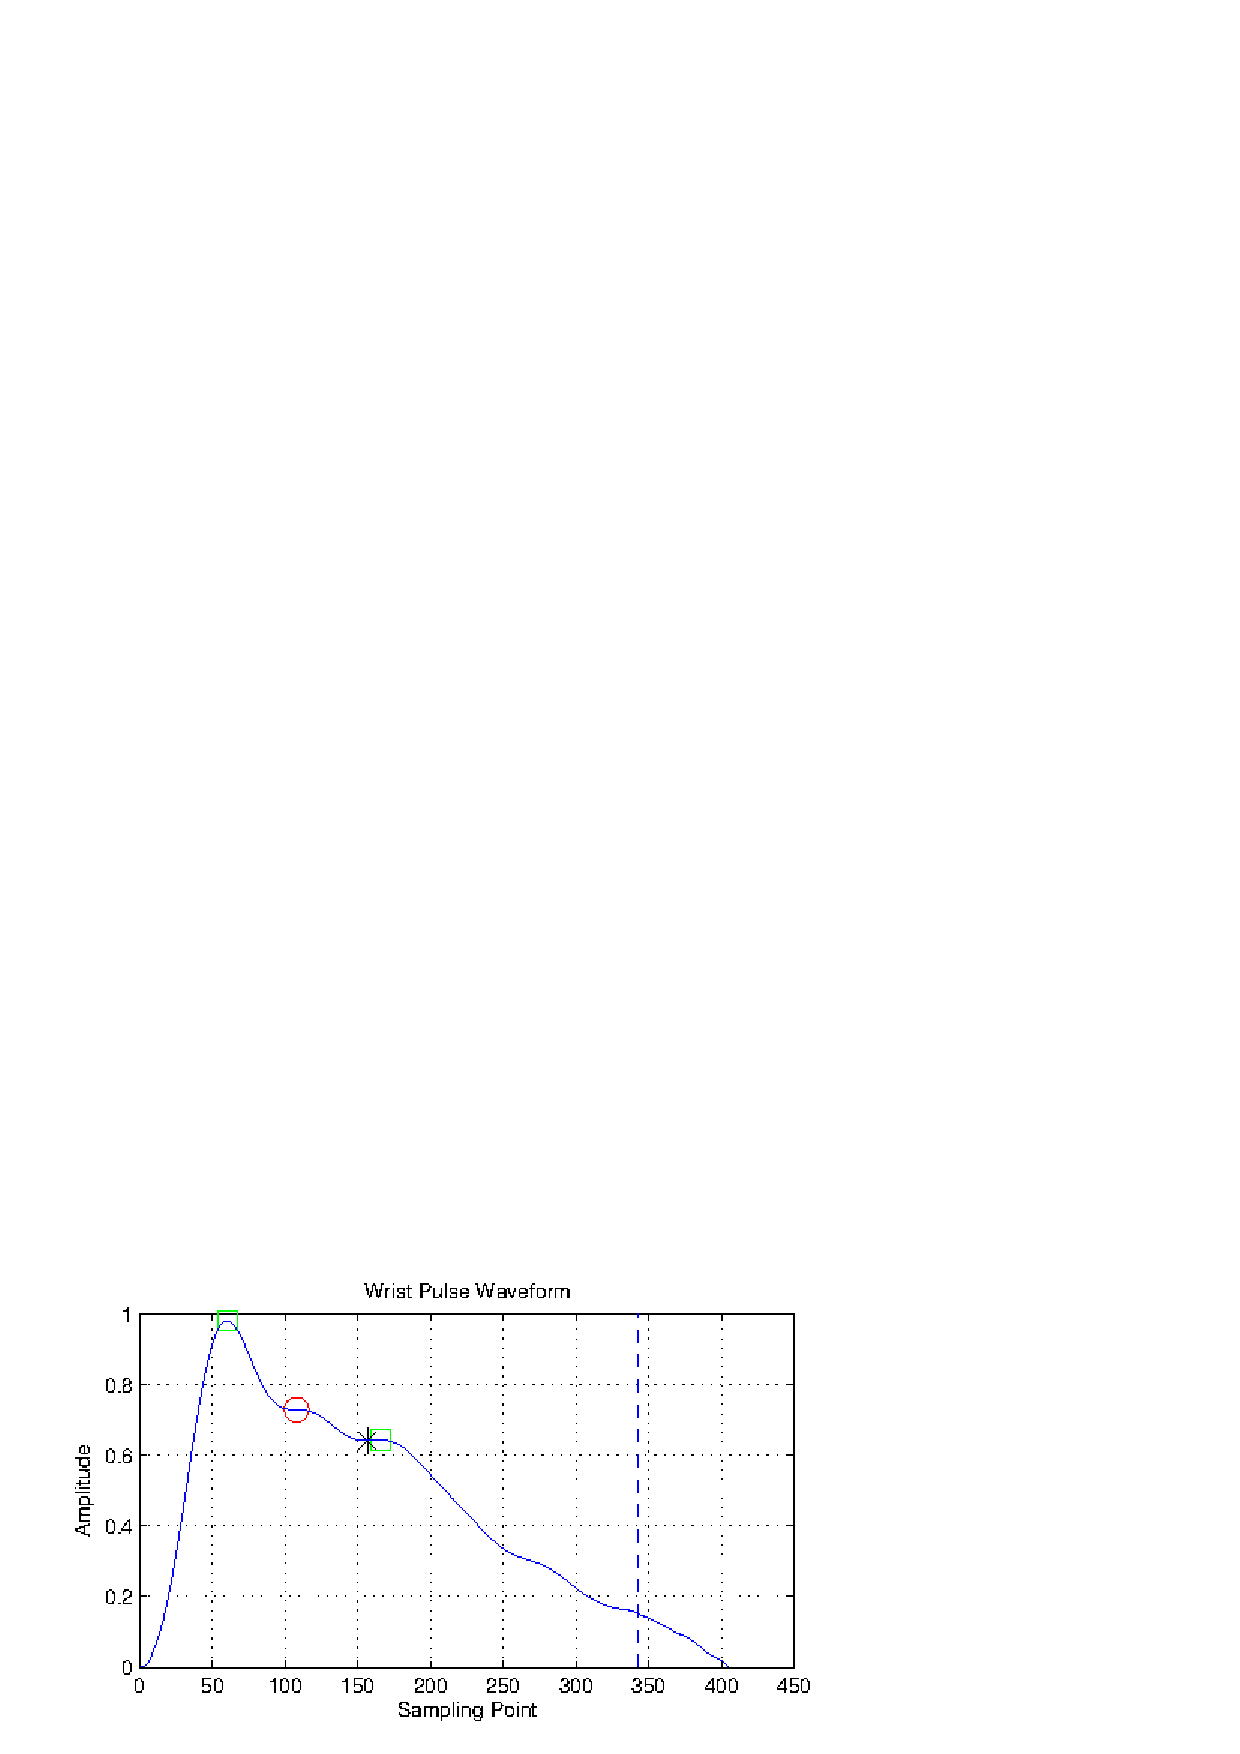
\includegraphics[width=0.7\textwidth]{hiddentidal}}\\
    \subfloat[The 1st-order
    difference]{\label{fig:1stdiff}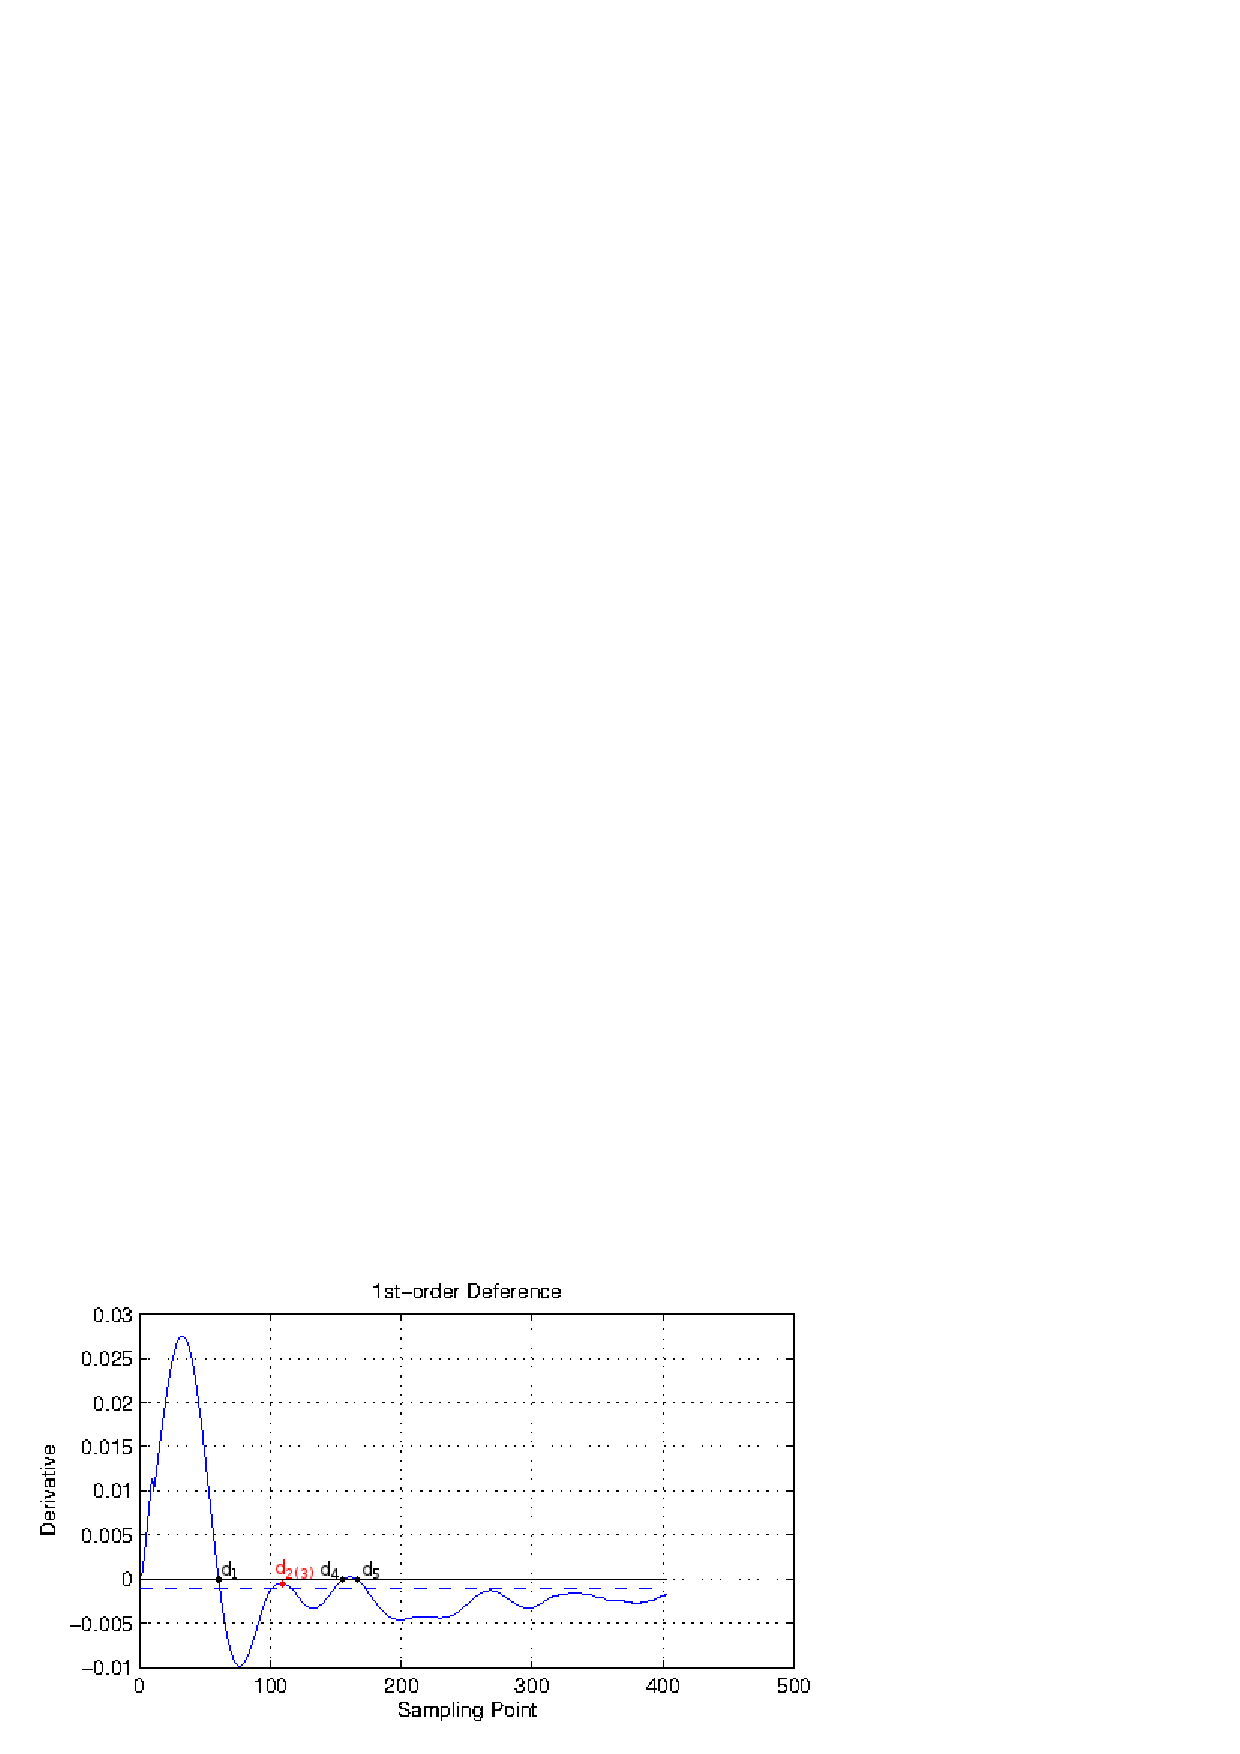
\includegraphics[width=0.7\textwidth]{1diff}}\\
    \subfloat[The 2nd-order
    difference]{\label{fig:2nddiff}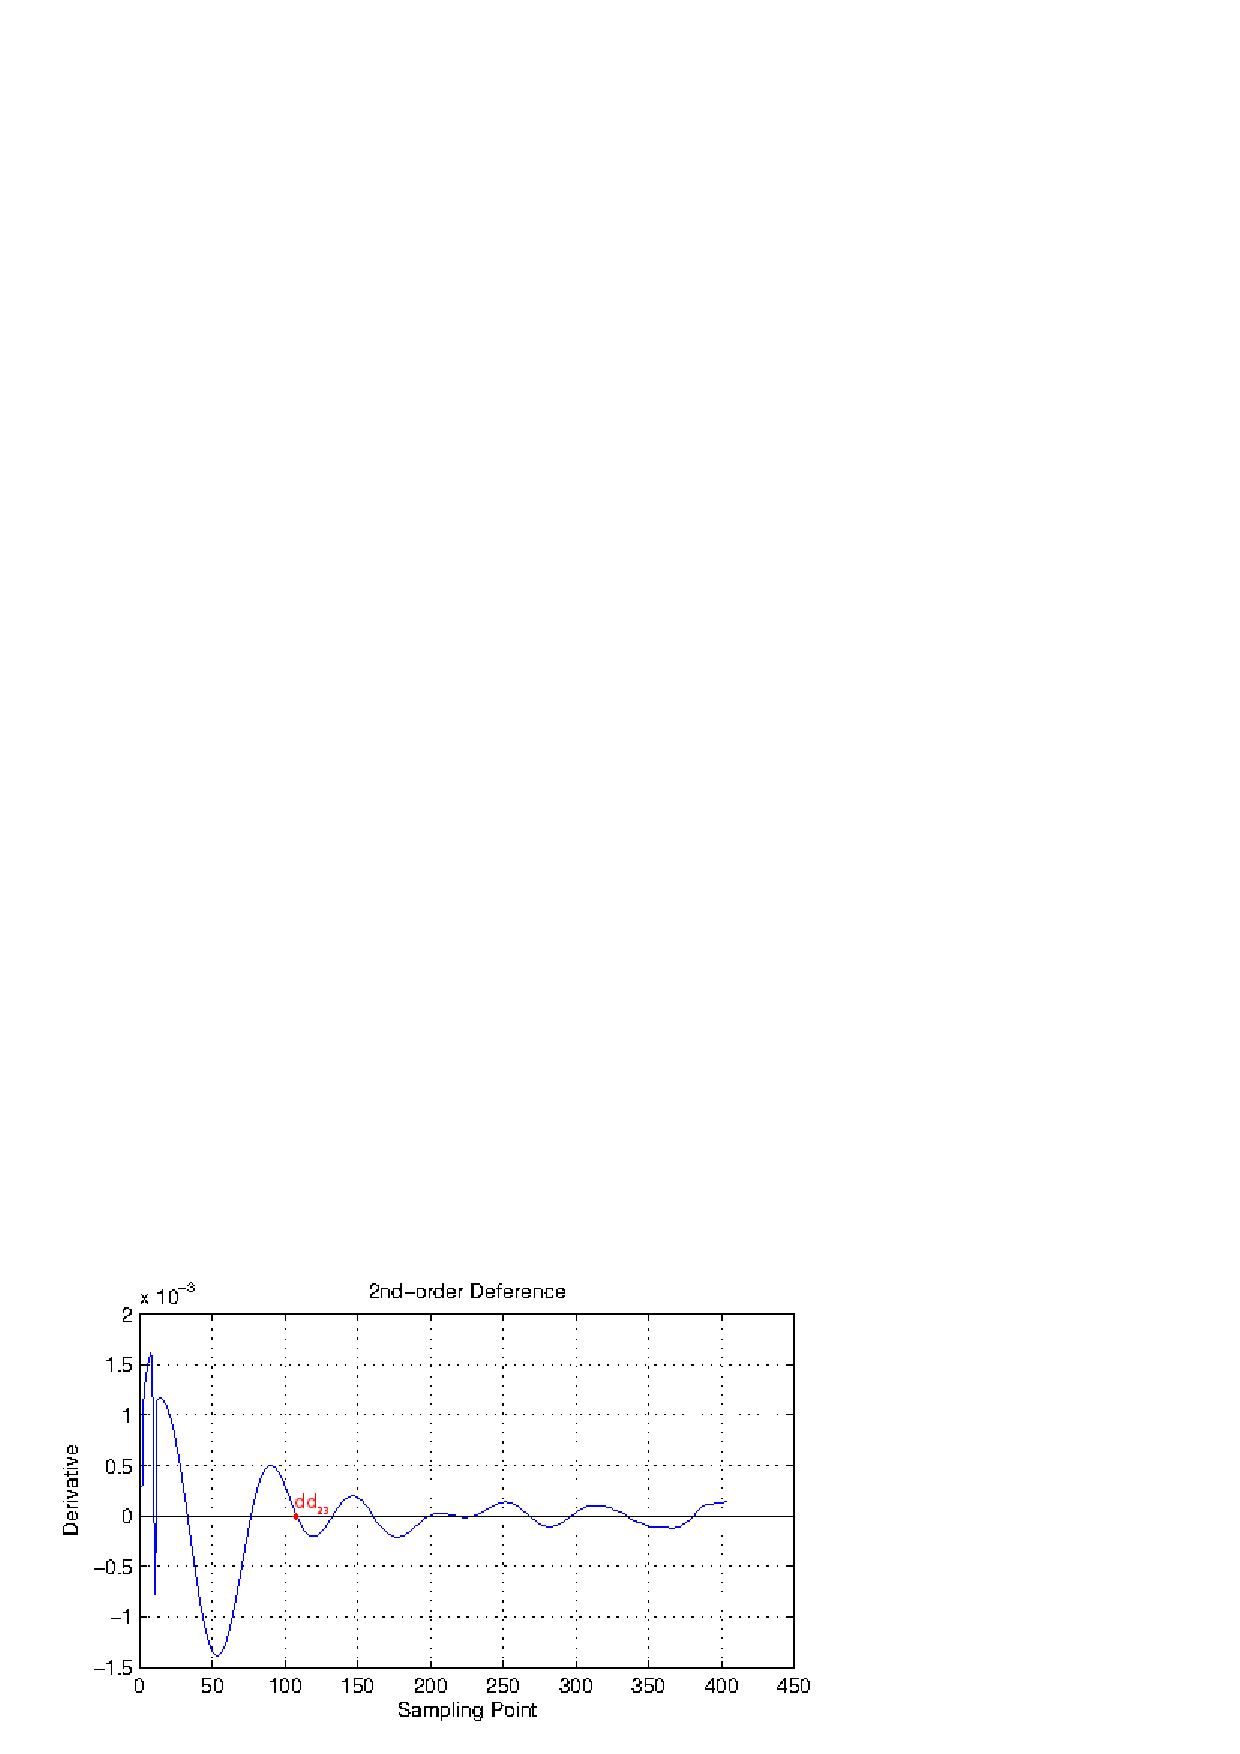
\includegraphics[width=0.7\textwidth]{2diff}}\\
    \caption{Illustration of the search of tidal wave}
    \label{fig:hiddentidal}
\end{figure}


\subsection{其他特征}

\todo{特征}
